%!TEX program = lualatex

\documentclass[parskip=full]{scrartcl}
\usepackage[a4paper, margin=20mm]{geometry}

\usepackage{scrlayer-scrpage}
\usepackage{bbm}
\usepackage{wrapfig}
\usepackage{paralist}
\usepackage{amsmath}
\usepackage{microtype}
\usepackage{xfrac}
\usepackage{tcolorbox}
\usepackage{tabularx}
\usepackage{hyperref}
\usepackage{multicol}
\usepackage{fancyvrb,newverbs,xcolor}
\usepackage{amssymb}
\usepackage{amsmath}
\usepackage{amsthm}
\usepackage{lmodern}
\usepackage{fontspec}
\usepackage{soul}
\usepackage[T1]{fontenc}
\usepackage[section]{placeins}

\tcbuselibrary{most}
\newfontfamily{\mono}{LigalexMono}
[Extension = .ttf, UprightFont = *-Text]

\definecolor{gbg}{rgb}{0.8, 1, 0.8}
\definecolor{bbg}{rgb}{0.85, 0.9, 1}
\definecolor{sep}{rgb}{0.5, 0.5, 0.5}
\definecolor{ksbg}{rgb}{0.92, 0.92, 0.92}
\definecolor{mkbg}{rgb}{0.92, 0.92, 0.5}
\def\columnseprulecolor{\color{sep}}
\sethlcolor{gbg}
\setlength{\columnseprule}{1pt}
\newcommand\pspara{\fontsize{13pt}{18pt}\selectfont}
\newcommand\psic{\fontsize{10pt}{18pt}\selectfont}
\newcommand\pstitle{\fontsize{21pt}{30pt}\selectfont}
% \newcommand{\fn}[1]{\hl{#1}}
\newcommand{\mk}[1]{\colorbox{mkbg}{#1}}
% \newcommand{\fnbox}[1]{\colorbox{gbg}{\parbox{1\textwidth}{#1}}}
\newcommand{\fn}[1]{#1}
\newcommand{\fnbox}[1]{\parbox{1\textwidth}{#1}}
\newcommand{\icbox}[1]{\colorbox{ksbg}{\parbox{1\textwidth}{\ic{#1}}}}
\newcommand{\ic}[1]{{\psic\mono#1}}
\newcommand{\icx}[1]{\psic\mono#1\pspara}
\newcommand{\icfn}[1]{{\psic\mono\fn{#1}}}
\newcommand{\e}[1]{\times 10^{#1}}

% \ifoot{Page \pagemark}
\cfoot{}
\ofoot{}

\hypersetup{
    colorlinks=true,
    linkcolor=teal
}

\newenvironment{lcverbatim}
 {\SaveVerbatim{cverb}}
 {\endSaveVerbatim
  \flushleft\fboxrule=0pt\fboxsep=.5em
  \colorbox{ksbg}{%
    \makebox[\dimexpr\linewidth-2\fboxsep][l]{\BUseVerbatim{cverb}}%
  }
  \endflushleft
}


\begin{document}

\begin{titlepage}

  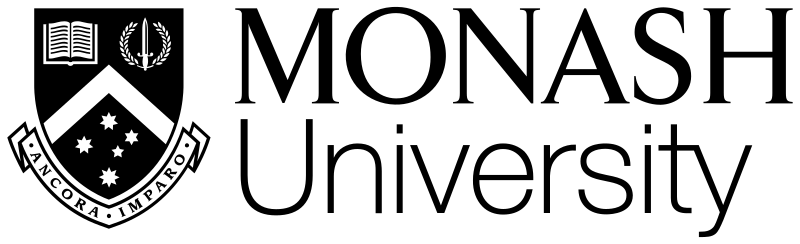
\includegraphics[width=0.25\linewidth]{monashlogo.png} \\
  
  
  \pstitle
  FIT2086 - Modelling for Data Analysis \\
  Assignment 2 Answer Attempts

  \vspace{2cm}
  
  \pspara
  Semester: 2023 - 2 \\
  Student Name: Xuanao Zhao \\
  Student ID: 33332835 \\
  Due Date: 16th OCT 2023 \\
  Due Date (Extended): 19th OCT 2023

  \vspace{5cm}

  % Final answers are highlighted in \fn{green}.

\end{titlepage}

% \begin{multicols*}{2}
\pspara
\section*{Question 1}
    \subsection*{Question 1.1}

    The 3 strongest predictors of Median value homes in descending order are \fn{
        (1) rm,
        (2) lstat and
        (3) ptratio}.
    
    This is because \fn{they have the lowest p-value among all predictors (i.e. $3.83 \e{-10}$, $6.26 \e{-9}$ and $2.73 \e{-6}$)}.

    \subsection*{Question 1.2}
    
    The threshold of acceptance of predictors is $\sfrac{\alpha}{p}$.

    There are 6 associated predictors (including the intercept) when using the Bonferroni procedure with $\alpha = 0.5$. They are \fn{
        (1) The intercept,
        (2) chas,
        (3) rm,
        (4) dis,
        (5) ptratio and
        (6) lstat}.

    \subsection*{Question 1.3}
    
    \fnbox{
        When the crime rate per capita increases by 1, the median house price will decrease by \$115.818.
        \\\\
        When the the suburb fronts the Charles River, the median house price will increase by \$4163.521.
    }

    \subsection*{Question 1.4}

    Let $x_1, x_2, x_3, x_4, x_5$ and $x_6$ be the estimators of \ic{chas}, \ic{nox}, \ic{rm}, \ic{dis}, \ic{ptratio} and \ic{lstat} in respective order, let $\hat{y}$ be the outcome \ic{medv}.

    The final regression equation is \\
    \\
    \fnbox{\[\begin{split}
        \mathbb{E}[\hat{y}] \; \approx \; & 29.19 + 4.60x_1 - 17.38x_2 + 4.82x_3 + 0.94x_4 - 0.96x_5 - 0.49x_6
    \end{split}\]}

    \subsection*{Question 1.5}

    <Place Holder>
    % The predictor ``Nitric oxide concentration (i.e. \ic{nox})'' is negatively correlated with the outcome. Since nitric oxide concentration is a bioproduct of living organisms (Roszer, T), therefore planting more tree

    \subsection*{Question 1.6}

    \mk{MARK}

    The \ic{predict} function yields the following result:
    
    \begin{lcverbatim}
      fit      lwr      upr
1 21.9196 20.30209 23.53712
    \end{lcverbatim}
    
    This means, that \fn{we are 95\% confident that the actual median value is between \$20302.09 and \$23537.12}.

    \subsection*{Question 1.7}

    \mk{MARK}
    
    <Place Holder>
\section*{Question 2}
    \subsection*{Question 2.1}

    There are a total of 7 leaves.

    The variables used in the tree are
    \begin{inparaenum}[(1)]
        \item Thallium scanning results (i.e. \ic{THAL}),
        \item Chest pain type (i.e. \ic{CP}),
        \item Number of major vessels colored by fluoroscopy (i.e. \ic{CA})
        \item Exercise induced angina (i.e. \ic{EXANG}) and
        \item Age of patient in years (i.e. \ic{AGE}).
    \end{inparaenum}

    \subsection*{Question 2.2}
    
    \autoref{fig:2_2_tree} shows an annotated plot of decision tree, where each leaf has 3 information notated, they are
    \begin{inparaenum}[(1)]
        \item a character of ``Y'' or ``N'' for estimated prediction of the target
        \item a ratio between ``Y'' and ``N'' of target that fulfills this leave's condition found in the sample and
        \item a percentage value showing the estimated probability of the target is ``Y'' for a certain leave, calculated using the ratio.
    \end{inparaenum}.

    As shown by the figure, predictors \ic{THAL} and \ic{CA} are relatively deterministic when determining present of heart disease. When \ic{THAL} is other then \ic{Normal}, the estimated probability of having a heart diseases increases from $24.2858\%$ to $75.8333\%$; Similarly, when \ic{THAL} is \ic{Normal}, but \ic{CA} is greater or equal to $0.5$, the estimated probability of having a heart diseases increases from $15.4472\%$ to $88.2353\%$.
    
    Other factors such as \ic{EXANG} and \ic{AGE} are also a factor, but they are multiple layer of factors under to filter out the lower estimated probability of heart diseases under anomalous \ic{THAL} (i.e. other than \ic{Normal} for \ic{THAL}), just the probability may be slightly lower.
    
    \subsection*{Question 2.3}
    
    See \autoref{fig:2_2_tree} for annotated tree.

    \begin{figure}
        \centering
        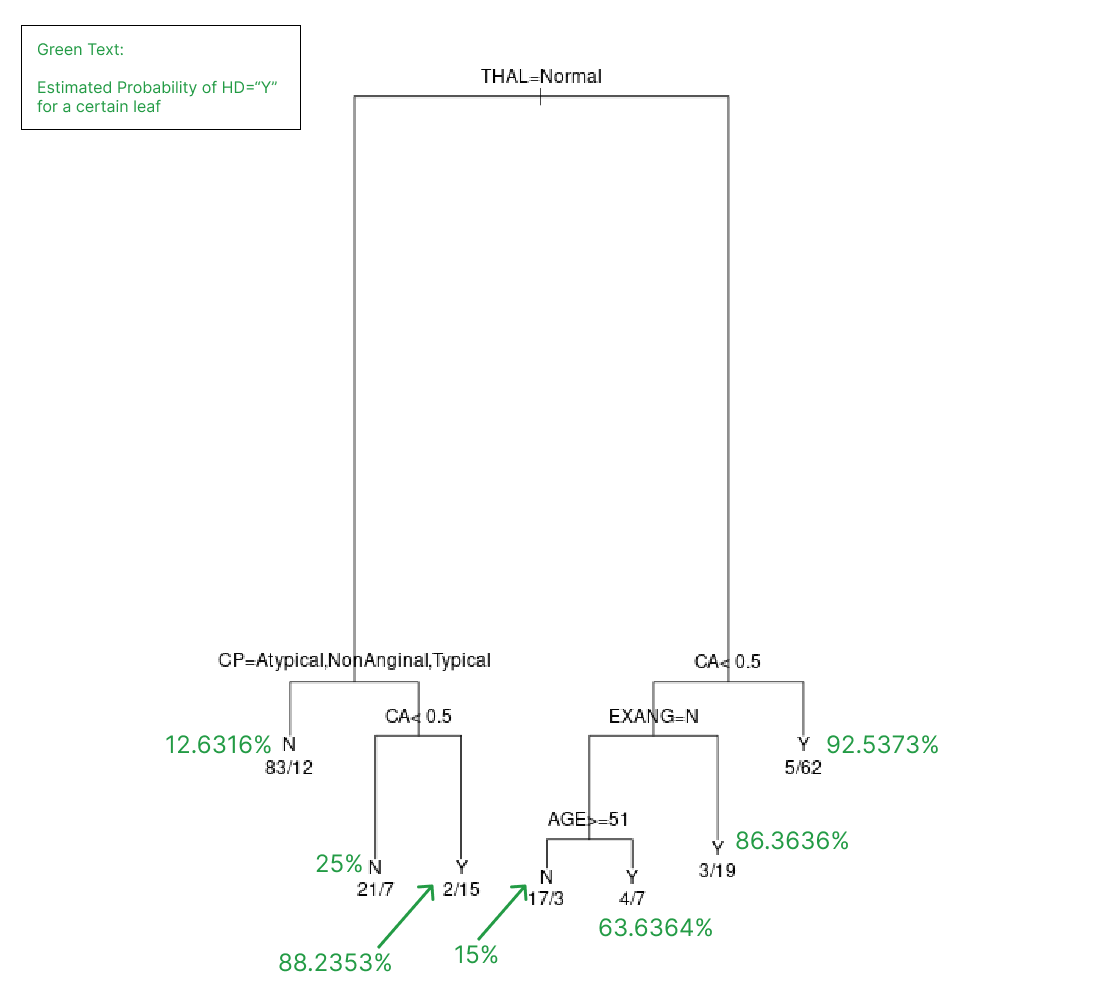
\includegraphics[width=0.7\linewidth]{diagrams/annotated.png}
        \caption{Cross Validated Decision Tree for Heart Disease.}
        \label{fig:2_2_tree}
    \end{figure}

    \subsection*{Question 2.4}
    
    According to the tree, the combination of predictor results will result in the highest estimated probability of heart diseases are a patient with anomalous \ic{THAL} reading and \ic{CA} of greater or equal to $0.5$, the estimated probability of this leaf is $92.5357\%$.

    \subsection*{Question 2.5}
    
    \mk{MARK}

    The most important predictor in terms of coefficient is \ic{CP} with one of its value contributing -1.8903 units to the model.

    The most important predictor in terms of p-value is \ic{CA}, with a p-value of $1.14\e{-5}$.

    \subsection*{Question 2.6}

    Let $p_{\text{AT}}$, $p_{\text{NA}}$ and $p_{\text{T}}$ be the categorical predictor of \ic{CP} with value \ic{Atypical}, \ic{NonAnginal} and \ic{Typical} respectively. When non of the predictor variable is 1, it represents the value of \ic{Asymptomatic}.

    Let $t_{\text{N}}$ and $t_{\text{R}}$ be the categorical predictor of \ic{THAL} with value \ic{Normal} and \ic{Fixed.Defect} respectively. When non of the predictor variable is 1, it represents the value of \ic{Reversible.Defect}.

    Let $r$, $o$ and $a$ be the predictor of \ic{THALACH}, \ic{OLDPEAK}, \ic{CA} respectively. (letter $r$ representing Rate)

    Let $\hat{y}$ be the outcome of \ic{HD}.

    The final regression model is

    \[\begin{split}
        \mathbb{E}[\hat{y}] = \; &
          2.7405
        - 1.1859p_{\text{AT}}
        - 1.8903p_{\text{NA}}
        - 1.8530p_{\text{T}}
        - 0.0235r
        + 0.5763o \\ &
        + 1.0985a
        - 0.3253t_\text{N}
        + 1.4594t_\text{R}
    \end{split}\]

    \subsection*{Question 2.7}
    
    
    \begin{figure}
        \centering
        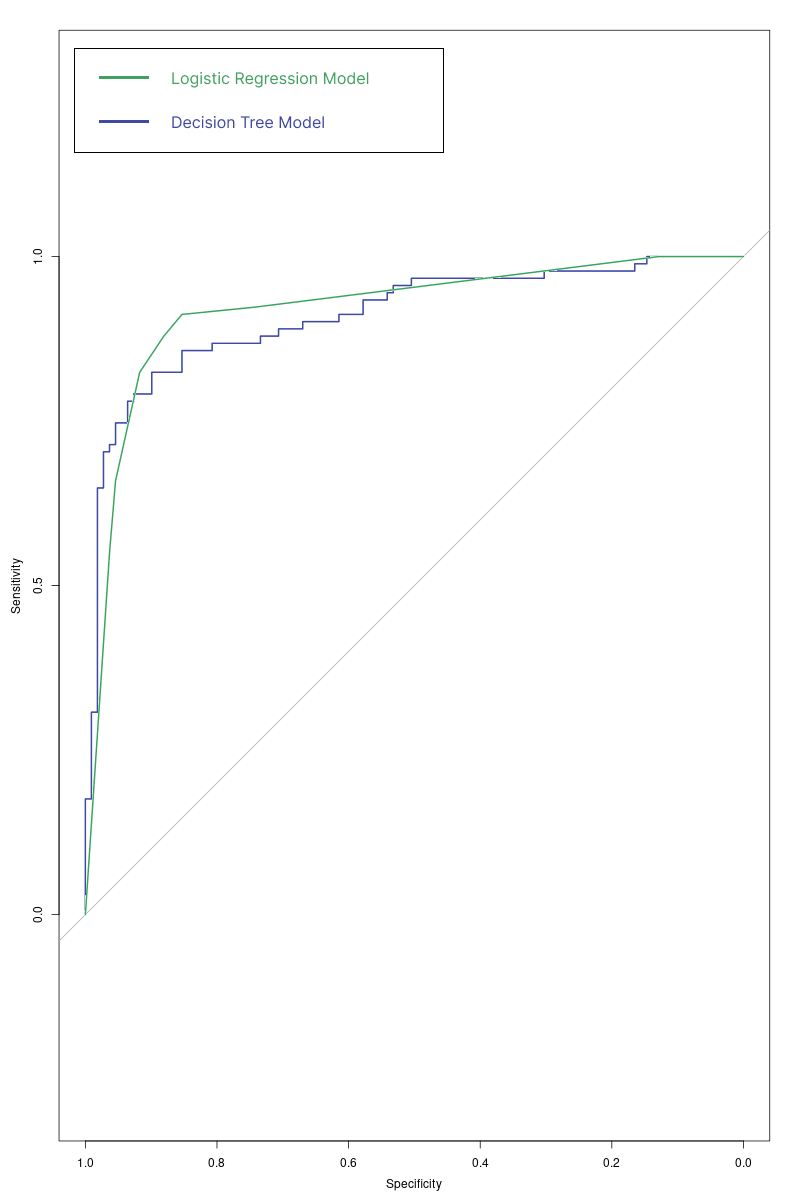
\includegraphics[width=0.9\linewidth]{diagrams/comp_test.png}
        \caption{Prediction Statistics Comparison for Tree Model and Logistic Regression Model.}
        \label{fig:2_7_fig}
    \end{figure}

    Shown by \autoref{fig:2_7_fig}, both model has reasonably similar accuracy, while the Decision Tree model is more accurate then the logistic model in the cental area.

    \subsection*{Question 2.8}
    
    <Place Holder>

    \subsection*{Question 2.9}
    
    <Place Holder>

    
\section*{Question 3}
    \subsection*{Question 3.1}
    
    <Place Holder>

    \subsection*{Question 3.2}
    
    <Place Holder>

    \subsection*{Question 3.3}
    
    <Place Holder>

    \subsection*{Question 3.4}
    
    <Place Holder>

    \subsection*{Question 3.5}
    
    <Place Holder>

    \subsection*{Question 3.6}
    
    <Place Holder>

    \subsection*{Question 3.7}
    
    <Place Holder>

    \subsection*{Question 3.8}
    
    <Place Holder>

    \begin{center}
        <End of Document>
    \end{center}
% \end{multicols*}
\end{document}

